\documentclass[12pt]{article}
%\usepackage{times}


\usepackage{parskip}
\usepackage{enumitem} %fix spaces on lists
\usepackage[ruled,vlined]{algorithm2e}
\usepackage{float}
\usepackage{graphicx}
\usepackage{url}
\usepackage{array}
\usepackage{booktabs}

\usepackage{xstring}

%\usepackage[square,authoryear]{natbib}

\usepackage[margin = 1cm]{geometry}
%\geometry{
%	paper=letterpaper, % Change to letterpaper for US letter
%	inner=1.5in, % Inner margin
%	outer=1in, % Outer margin
%	bindingoffset=0in, % Binding offset
%	top=1in, % Top margin
%	bottom=1in, % Bottom margin
%	%showframe,% show how the type block is set on the page
%}

\title{CS 6965 - Project 1}
\author{Maks Cegielski-Johnson}

\newcommand{\problem}[2]{
	\subsection*{#1}
	\textbf{#2}
}

\newcommand{\image}[3]{
\begin{figure}[H]
	\centering
	\includegraphics[scale=#3]{figures/#1}
	\caption{#2}
	\label{#1}
\end{figure}
}

\newcommand{\doubleimage}[5]{
\begin{figure}[H]
	\centering
	\begin{minipage}{#5\textwidth}
		\centering
		\includegraphics[width=.5\linewidth]{figures/#1}
		\caption{#2}
		\label{#1}
	\end{minipage}%
	\begin{minipage}{#5\textwidth}
		\centering
		\includegraphics[width=.5\linewidth]{figures/#3}
		\caption{#4}
		\label{#3}
	\end{minipage}
\end{figure}
}



%%%%%%%%%%%%%%%%%%%%%%%

%\hypersetup{pdftitle=\ttitle} % Set the PDF's title to your title
%\hypersetup{pdfauthor=\authorname} % Set the PDF's author to your name
%\hypersetup{pdfkeywords=\keywordnames} % Set the PDF's keywords to your keywords

%%%%%%%%%%%%%%%%%%%%%%%



\begin{document}
\maketitle

\problem{Q1}{What is the effect of increasing interval overlap parameter on the final graph in the visualization?}


\doubleimage{q1-overlap20}{20\% Overlap}{q1-overlap80}{80\% Overlap}{0.5}

Firstly, as we can see from the two figures, there are fewer clusters when the overlap is set to 80\% than there are with 20\% overlap. Secondly, upon inspecting the clusters, it becomes apparent that the clusters in Figure \ref{q1-overlap80} have larger membership than those in Figure \ref{q1-overlap20}. This is not surprising due to the pigeonhole principle. Having a larger overlap means more points are members of multiple clusters. 

\problem{Q2}{What is the effect of increasing number of interval parameter on the final graph in the visualization?}

\doubleimage{q1-overlap80}{80\% Overlap and 15 Intervals}{q2-interval30}{80\% Overlap and 30 Intervals}{0.5}

As seen in the figures, increasing the number of intervals from 15 to 30 increases the number of clusters from 18 to 39 clusters, as well as changing the color scale from $[lightgreen, red]$ to $[blue,red]$, indicating the addition of more clusters. There is also a larger amount of \textit{small} clusters, with membership less than 100. This is visually indicated my the larger amount of circles with small radius. 

\problem{Q3}{Why does the resulting graph contain two connected component?}

\doubleimage{q3-mapper}{Mapper visualization of bunny}{q3-bunny}{Original bunny point cloud}{0.5}

If we look at the original bunny point cloud Figure \ref{q3-bunny}, then we see that one of the ears is relatively far from the rest of the bunny. Since these points are far \textit{enough} away from the rest of the points, they end up in a disconnected cluster. 

\problem{Q4}{What does this modification do to my data? (Hint, what lens am I using for my data after the modification?)}

\doubleimage{q3-mapper}{Mapper visualization of bunny}{q4-lens}{Mapper visualization with lens}{0.5}

Changing the projection to $[1]$ projects our point cloud data onto an axis-aligned line for the second dimension (dimension with index 1), in this case mapping the data onto the $y$-axis. In other words, takes only the data in the $y$-dimension of our original point cloud (the height function in $y$ dimension)

\problem{Q5}{Does this modification help better capture the shape of the data? If yes, how?}

\doubleimage{q3-bunny}{Original point cloud of bunny}{q5-kmeans}{Mapper visualization with K-Means}{0.5}

Yes it does. There appears to be a clear section for the head, ears, body, tails, and legs. 

\problem{Q6}{Why are the results not necessarily identical?}

\doubleimage{q6-first}{First Run}{q6-second}{Second Run}{0.5}

The results are not identical because there is randomization during the initialization of the gradient descent. 

\image{q6-tsne}{t-SNE Pseudocode}{0.35}

This can be seen in Figure \ref{q6-tsne} on the line which randomly samples $\mathcal{Y}^{(0)}$ from $\mathcal{N}(0, 10^{-4} I)$. 


\problem{Q7}{What is the difference between the resulting using Spectral Embedding in comparison to the results using t-SNE?}

\doubleimage{q6-first}{Mapping with t-SNE}{q7-spectral}{Mapping with Spectral Embedding}{0.5}

There is a smaller number of connected components in the Spectral Embedding graph than in the t-SNE graph, with most of the connected components being the same size as in t-SNE except for one which is significantly larger. 


\problem{Q8}{What is your modification and its effect on the data?}
\doubleimage{q7-spectral}{Spectral Embedding, dimension 2}{q8-spectral3}{Spectral Embedding, dimension 3}{0.5}

Since we were asked the only change the parameters of the spectral embedding, I left the mapper parameters the same. I increased the dimension of the projected subspace from 2 to 3, with the resulting graph in Figure \ref{q8-spectral3}. The result was that the large connected component from the original spectral embedding with dimension 2 being split up to a set of few clusters, splitting up the numbers much better. There was still a little bit of noise in some of the groups, and two groups of different digits were connected by one noisy cluster (the yellow/orange group in the bottom left, above the cyan group in Figure \ref{q8-spectral3}).

I also tried setting the subspace to 4 dimensions, but this didn't have any interesting results.

\problem{Q9}{Custom dataset}

For my dataset I reused my Spotify Chart dataset which I used for the CS 6630 (data visualization) final project\footnote{\url{https://makscj.github.io/visualization-project/}} last semester. The data represents all of the songs that were in the Spotify Weekly Global Top 200 throughout 2017, and some relevant information about these songs. One specific set of data associated with each song is it's track features, which is a set of extracted values describing different aspects of the track, all computed and provided by Spotify. 

\begin{itemize}

\item \textbf{Acousticness}

A confidence measure from 0.0 to 1.0 of whether the track is acoustic. 1.0 represents high confidence the track is acoustic.

\item \textbf{Danceability}

Danceability describes how suitable a track is for dancing based on a combination of musical elements including tempo, rhythm stability, beat strength, and overall regularity. A value of 0.0 is least danceable and 1.0 is most danceable.

\item \textbf{Energy}

Energy is a measure from 0.0 to 1.0 and represents a perceptual measure of intensity and activity. Typically, energetic tracks feel fast, loud, and noisy. For example, death metal has high energy, while a Bach prelude scores low on the scale. Perceptual features contributing to this attribute include dynamic range, perceived loudness, timbre, onset rate, and general entropy.

\item \textbf{Instrumentalness}

Predicts whether a track contains no vocals. "Ooh" and "aah" sounds are treated as instrumental in this context. Rap or spoken word tracks are clearly "vocal". The closer the instrumentalness value is to 1.0, the greater likelihood the track contains no vocal content. Values above 0.5 are intended to represent instrumental tracks, but confidence is higher as the value approaches 1.0.

\item \textbf{Liveness}

Detects the presence of an audience in the recording. Higher liveness values represent an increased probability that the track was performed live. A value above 0.8 provides strong likelihood that the track is live.

\item \textbf{Speechiness}

Speechiness detects the presence of spoken words in a track. The more exclusively speech-like the recording (e.g. talk show, audio book, poetry), the closer to 1.0 the attribute value. Values above 0.66 describe tracks that are probably made entirely of spoken words. Values between 0.33 and 0.66 describe tracks that may contain both music and speech, either in sections or layered, including such cases as rap music. Values below 0.33 most likely represent music and other non-speech-like tracks.

\item \textbf{Valence}

A measure from 0.0 to 1.0 describing the musical positiveness conveyed by a track. Tracks with high valence sound more positive (e.g. happy, cheerful, euphoric), while tracks with low valence sound more negative (e.g. sad, depressed, angry).

\item \textbf{Loudness}

Average Decibel measure of the song.  

\end{itemize}

I then use these features and over 1000 songs in conjunction with t-SNE and the keppler mapper to visualize the data. Although not in the scope of this assignment, the resulting graph could be incorporated with my visualization from CS 6630 to allow for better user interaction to see if any patterns can be discovered. 

Since the point-cloud is more or less artificially induced through other machine learning tools, the expected outcome of the keppler-mapper visualization is unknown. Playing with the parameters results in different visualizations, all of which are interesting and seem to provide some insight to the data. 

Below are several of the results displayed for different parameters, with a referenece to the particular HTML file which can be viewed in more detail. 

\begin{table}[H]
	\centering
\begin{tabular}{|c|c|c|c|}
	\hline
	\multicolumn{2}{c}{DBSCAN} & \multicolumn{2}{c}{DBSCAN}\\ \hline
	\multicolumn{2}{c}{\textit{music\_vis\_1.html}} & \multicolumn{2}{c}{\textit{music\_vis\_2.html}}\\ \hline
n\_components & 3 & n\_components & 2\\\hline
perplexity & 40 & perplexity & 30\\\hline
eps & 0.4 & eps & 0.6\\\hline
min\_samples & 15 & min\_samples & 15\\\hline
nr\_cubes & 15 & nr\_cubes & 15\\\hline
overlap\_perc & 0.5 & overlap\_perc & 0.5\\\hline
	\multicolumn{2}{c}{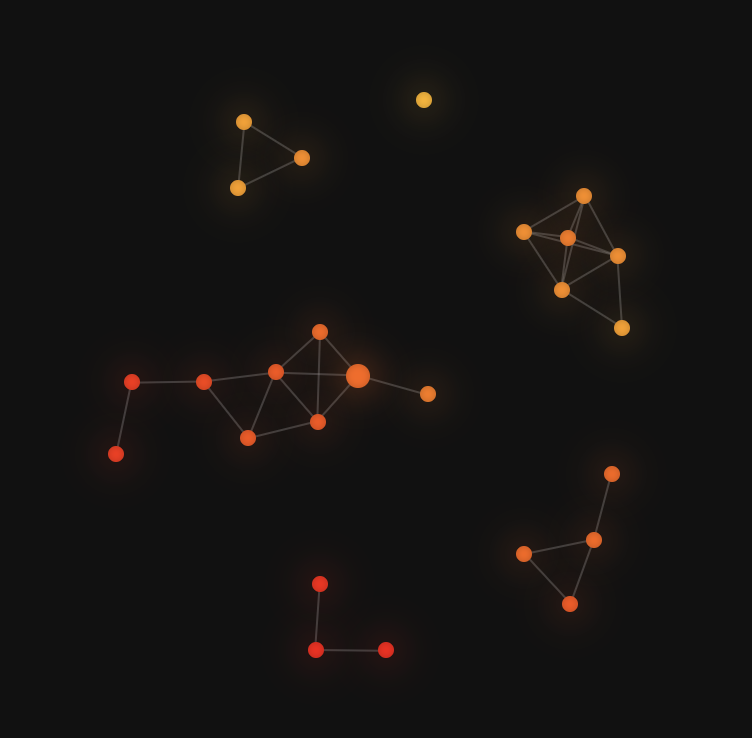
\includegraphics[scale=0.48]{figures/mydata1}} & 	\multicolumn{2}{c}{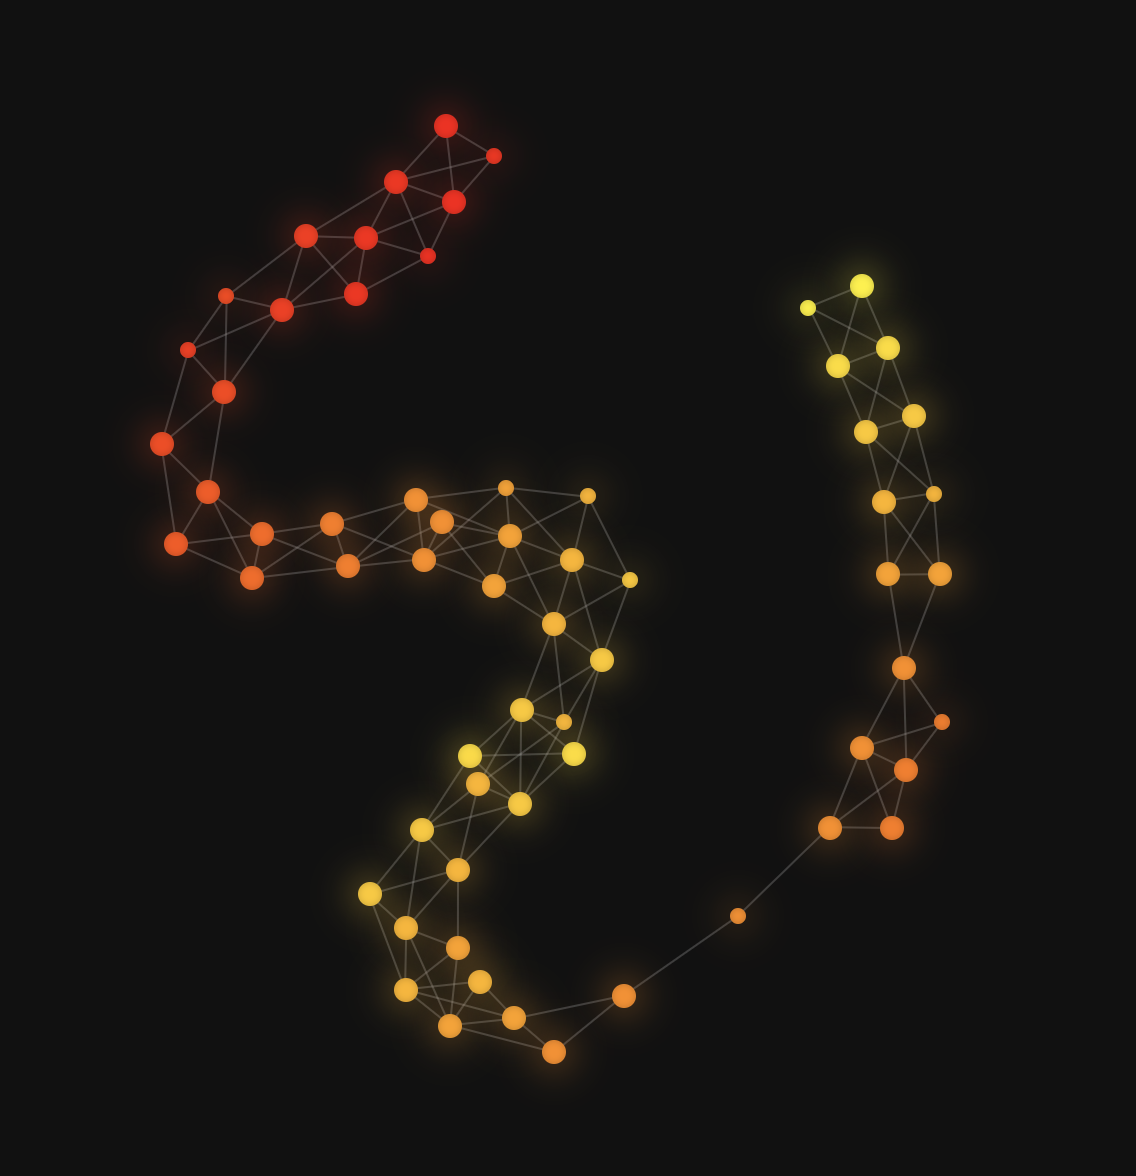
\includegraphics[scale=0.3]{figures/mydata2}}\\\hline
	\multicolumn{2}{c}{DBSCAN} & \multicolumn{2}{c}{K-MEANS}\\ \hline
	\multicolumn{2}{c}{\textit{music\_vis\_3.html}} & \multicolumn{2}{c}{\textit{music\_vis\_4.html}}\\ \hline
n\_components & 2 & n\_components & 2\\\hline
perplexity & 40 & perplexity & 30\\\hline
eps & 0.3 & n\_clusters & 2\\\hline
min\_samples & 10 &  & \\\hline
nr\_cubes & 20 & nr\_cubes & 20\\\hline
overlap\_perc & 0.2 & overlap\_perc & 0.2\\\hline
	\multicolumn{2}{c}{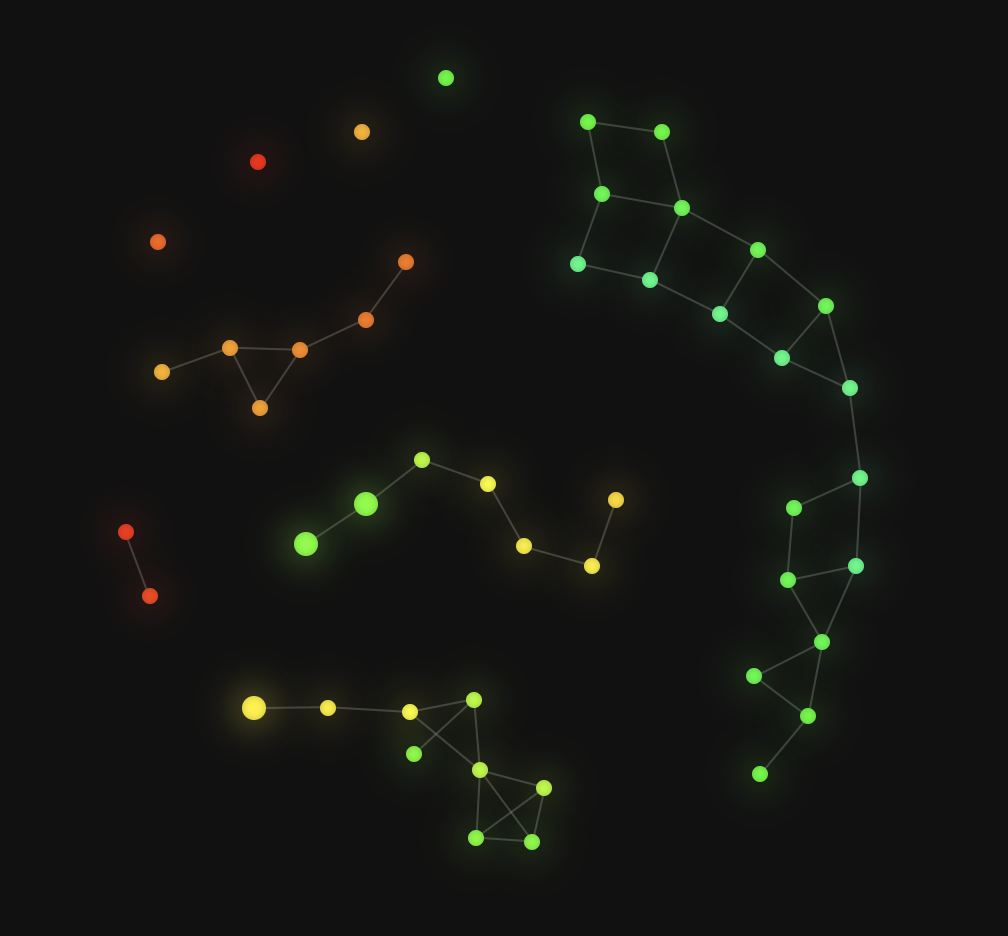
\includegraphics[scale=0.4]{figures/mydata3}} & 	\multicolumn{2}{c}{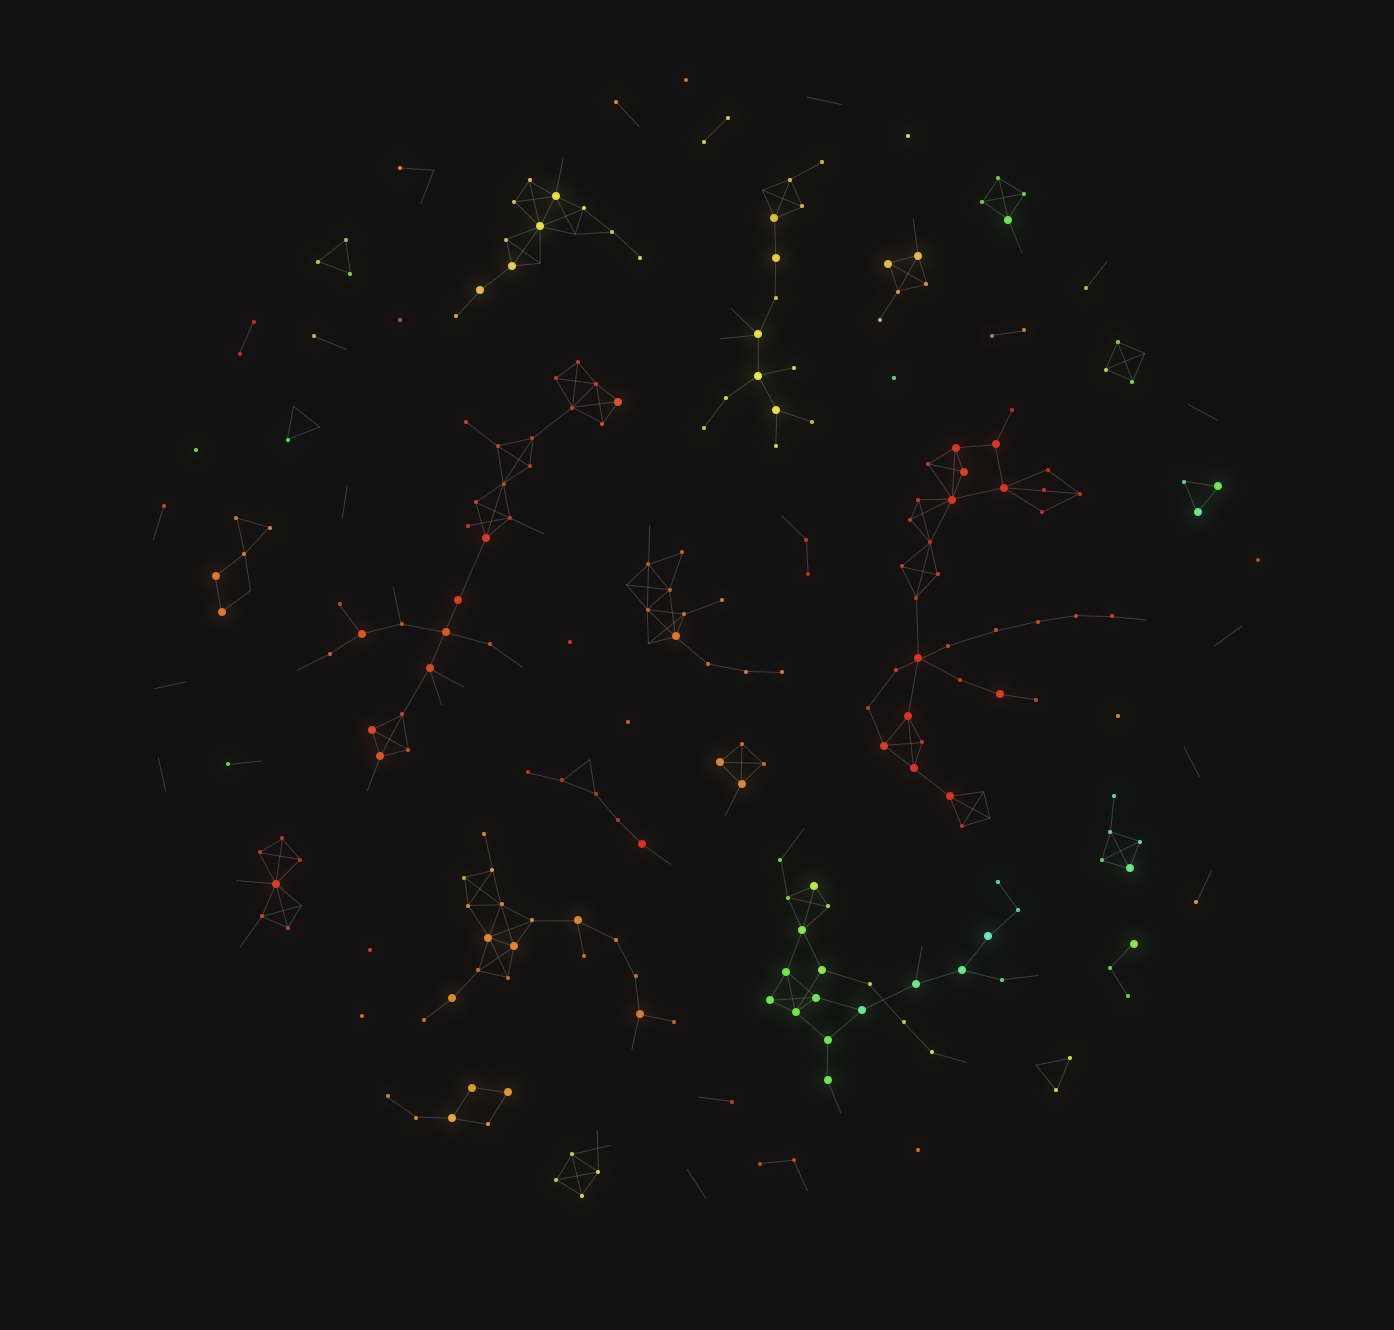
\includegraphics[scale=0.28]{figures/mydata4}}
	
\end{tabular}
\end{table}

\end{document}


%%% Local Variables:
%%% mode: latex
%%% TeX-master: t
%%% End: